\section{Problem statement}
\frame{\sectionpage}
\begin{frame}{Eye description}
The eye is the organ of vision; it allows the conversion of light into impulses in neurons.
\begin{center}
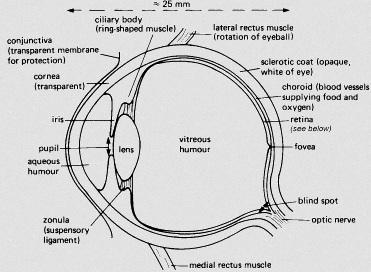
\includegraphics[width=.7\linewidth]{Eye.jpg}
\end{center}
\tiny{source: \url{http://academia.hixie.ch/bath/eye/home.html}}
\end{frame}

\begin{frame}{Eye description}
Aqueous humor: produced by the ciliary epithelium.
$\rightarrow$ drains into the Schlemm's canal.\\
Pressure produced: the intra-ocular pression (IOP).
\begin{center}
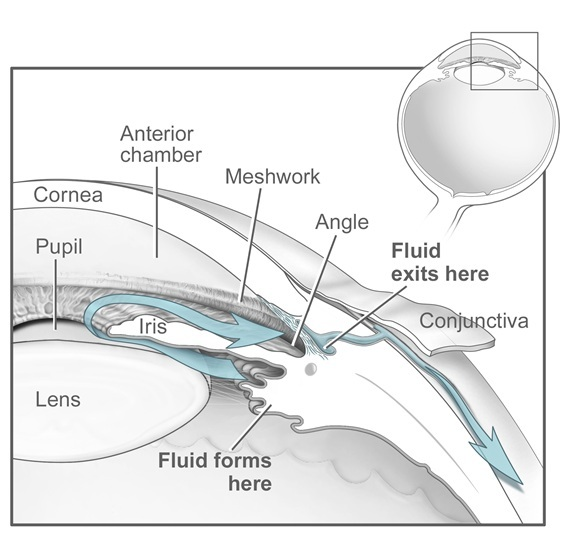
\includegraphics[width=.5\linewidth]{Humor.jpg}
\end{center}


\end{frame}

\begin{frame}{IOP}
IOP : 10 -- 22 mmHg for healthy humans (average : 16 mmHg)
\begin{itemize}
\item inflates the globe of the eye.
\item experimental measure (tonometry) takes into account the thickness of the cornea.
\end{itemize}
%
%
%Note that its value can be measured by tonometry by taking into account the thickness of the cornea. A fine jet of air is directed toward the cornea.
\begin{center}
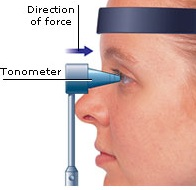
\includegraphics[scale=.6]{Tonometry.jpg}\\
\tiny{source: \url{http://www.aviva.co.uk/health-insurance/home-of-health/medical-centre/medical-encyclopedia/entry/test-tonometry/}}
\end{center}
\only<2>{\begin{center}
\ALERT{High IOP $\Rightarrow$ major risk for vision loss}.
\end{center}}
\end{frame}

\begin{frame}{Glaucoma}
%The glaucoma, also called the silent thief of sight, is known as the second leading cause of blindness worldwide (1 in 40 adults over 40 years old).
%\newline
%\\
\begin{itemize}
\item Second leading cause of blindness worldwide (1 in 40 adults over 40 years old)\footnote{\textit{Relative roles of risk factors in the evaluation of a glaucoma suspect : clinical perspective and mathematical modeling},Geffen, Guidoboni, Harris \textit{et al}}
\end{itemize}
% Until now, the major risk for glaucoma is the elevated IOP but it is neither required nor enough to actually contract the disease:\\
Elevated IOP : major risk for glaucoma, but :
\begin{itemize}
\item a patient with an elevated IOP may never contract glaucoma.
\item a patient could have a glaucoma even though his/her IOP is low
\end{itemize}
\begin{center}
\alert{ 25 \% of IOP-treated patients progress to blindness}

\end{center}

\end{frame}

\begin{frame}{Glaucoma}
Group of ocular disorders with multi-factorial etiology united by a clinically characteristic optic neuropathy accompanied by a vision loss.
%\newline
%\\
There are two kinds of diagnostics: \\
\begin{itemize}
\item<2-> a morphological damage
\item<3->a functional damage (decrease of the visual field)
\end{itemize}
\only<2>{
\begin{center}
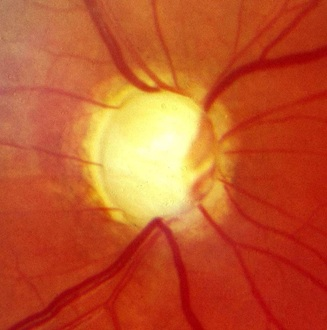
\includegraphics[scale=.5]{Morphological.jpg}\\
\tiny{Glaucomateous optic nervehead demonstrating increased cup to disc ratio;}
\end{center}
Glaucoma damages the optical nerve head, where the optical nerve and blood vessels enter the retina.}
\only<3>{

\begin{center}
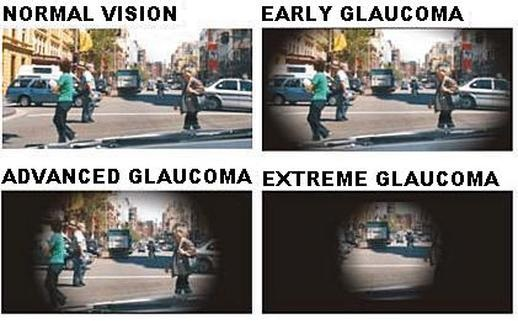
\includegraphics[scale=.5]{Glaucoma.jpg}\\
\tiny{source: \url{http://www.swisscompleteeyecare.com/uploads/3/6/3/8/3638142/8901258.jpg?520}}

\end{center}}
\only<4>{
\begin{center}
\ALERT{
Even though IOP is certainly not the only risk factor in glaucoma, \\ the IOP remains the only parameter we can act on, \\ either by surgery or with medications.
}\end{center}}
\end{frame}

\begin{frame}[shrink=5]{Treatment}

The medications have two effects:
%: either decrease the secretion of aqueous humor or increase the elimination of it. It is also possible to combine several treatments in order to decrease even more the IOP.
\newline
\\
\begin{tabular}{|c|c|}
\hline
Decrease the secretion & Increase the elimination \\
of aqueous humor &  of aqueous humor\\
\hline
beta-adrenergic receptor antagonists & Prostaglandin analogs \\
Alpha2-adrenergic agonists & Miotic agents \\
alpha agonists &  \\
Carbonic anhydrase inhibitors &  \\
\hline
\end{tabular}
\newline
\newline

{\bf Remarks:}

\begin{itemize}
 \item Several treatments may be combined to improve their efficiency.\\
 \item The drugs may work better on patients depending on their age, gender, ethnic group or other diseases like diabetes, hypertension ...
\end{itemize}



\end{frame}

\begin{frame}{Open questions?}

$\Rightarrow$Lack of knowledge\newline
-The mechanisms influencing glaucoma are not known yet.\newline
-The IOP is the only parameter we can measure.\newline
-Too many different factors whose contribution have to be weighed.\newline

$\Rightarrow$Math contribution\newline
-Statistic studies (useful but not enough to fully understand the phenomena since it differs from patient to patient)\newline
-Modeling the dynamic of the aqueous humor (link between the flow and the pressure) and the influence of the drugs

\end{frame}